% ---------------------------------------------------------------
% Auto-generated figure blocks. Copy the ones you need into the paper,
% or \input this whole file to see every figure at once.
%
% Requires in the preamble:  \usepackage{graphicx}
% ---------------------------------------------------------------

% ===== Main paper figures (6 figures) =====

% Benchmark band 1: strongest models (Accuracy)
% Question answered: Which models are the strongest on Accuracy?
\begin{figure}[t]
  \centering
  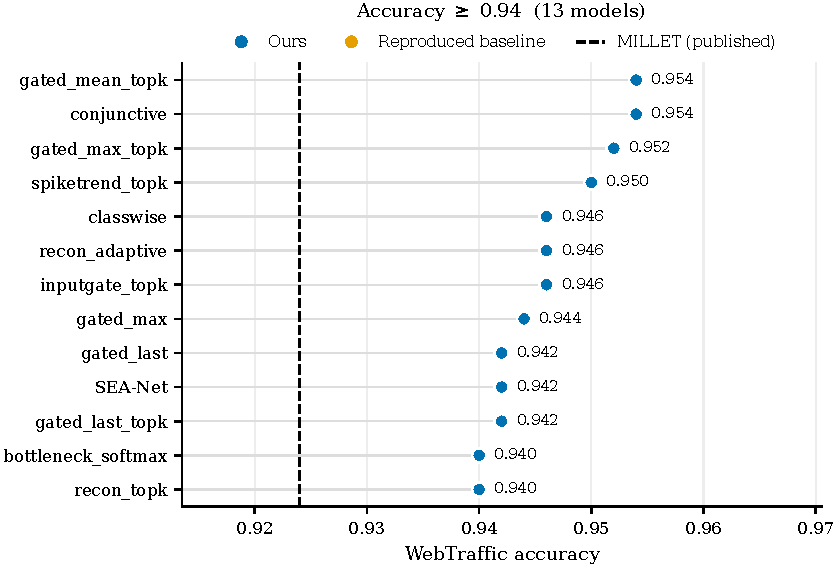
\includegraphics[width=\linewidth]{results/paper_figures/01_main_figures/fig1_benchmark_strongest_web_acc}
  \caption{Accuracy of the strongest models on WebTraffic (13 models, Accuracy $\geq$ 0.94). Bars are sorted best-first; blue marks models proposed in this work and orange our reproduction of the published backbones. Labels read \texttt{encoder\_\_pooling}, abbreviated, where sea\_ marks a component introduced here and mil\_ one reused unchanged from MILLET. The dashed line is the accuracy reported in the MILLET paper. Bands are disjoint, so each model appears in exactly one of Figures 1--3.}
  \label{fig:fig1_benchmark_strongest_web_acc}
\end{figure}

% Benchmark band 2: competitive models (Accuracy)
% Question answered: Which models are the competitive on Accuracy?
\begin{figure}[t]
  \centering
  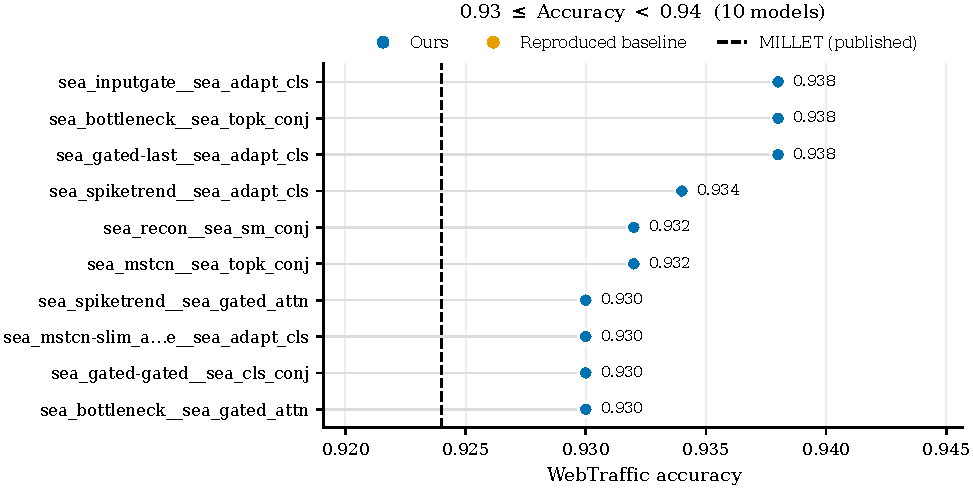
\includegraphics[width=\linewidth]{results/paper_figures/01_main_figures/fig2_benchmark_competitive_web_acc}
  \caption{Accuracy of the competitive models on WebTraffic (10 models, 0.93 $\leq$ Accuracy $<$ 0.94). Bars are sorted best-first; blue marks models proposed in this work and orange our reproduction of the published backbones. Labels read \texttt{encoder\_\_pooling}, abbreviated, where sea\_ marks a component introduced here and mil\_ one reused unchanged from MILLET. The dashed line is the accuracy reported in the MILLET paper. Bands are disjoint, so each model appears in exactly one of Figures 1--3.}
  \label{fig:fig2_benchmark_competitive_web_acc}
\end{figure}

% Accuracy vs Parameters (Pareto)
% Question answered: Does a smaller model stay competitive once parameters is taken into account?
\begin{figure}[t]
  \centering
  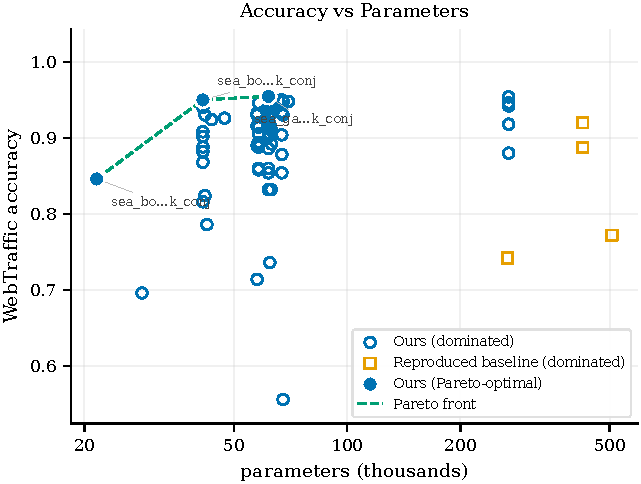
\includegraphics[width=\linewidth]{results/paper_figures/01_main_figures/pareto_web_acc_vs_params}
  \caption{WebTraffic accuracy against parameters (thousands). Filled markers joined by the dashed line are Pareto-optimal: no other model is both cheaper and better. Hollow markers are dominated and therefore never the right choice. Only Pareto-optimal models are labelled.}
  \label{fig:pareto_web_acc_vs_params}
\end{figure}

% Top-5 models across all metrics
% Question answered: Which of the top-5 models is preferable once every metric is considered?
\begin{figure*}[t]
  \centering
  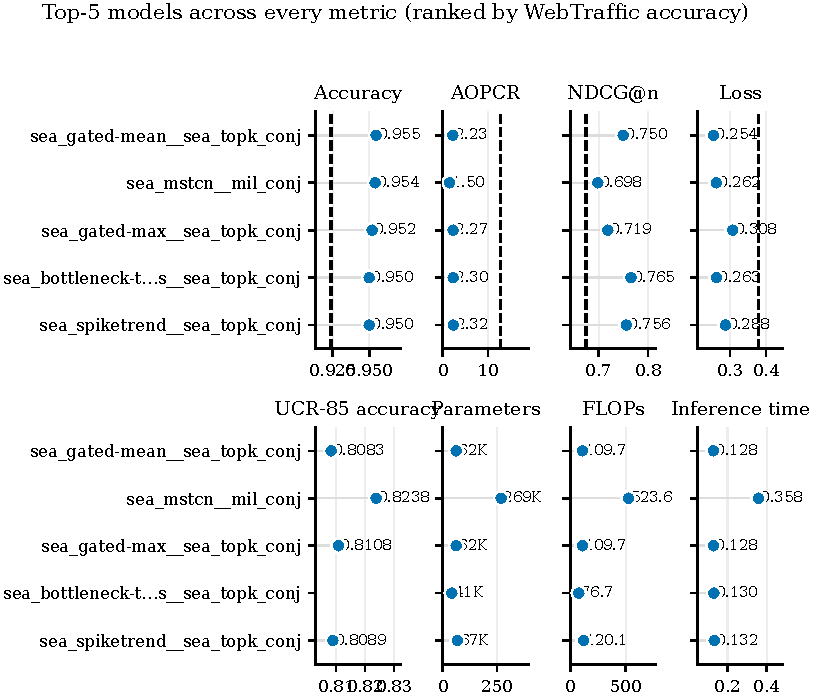
\includegraphics[width=\linewidth]{results/paper_figures/01_main_figures/topk5_multimetric}
  \caption{The top-5 models, ranked by WebTraffic accuracy, compared on every available metric. Panels share the same model order, so a single model can be followed across quality (accuracy, AOPCR, NDCG, loss) and cost (parameters, FLOPs, latency). Blue marks models proposed in this work.}
  \label{fig:topk5_multimetric}
\end{figure*}

% Critical difference diagram (accuracy)
% Question answered: Which differences in accuracy are statistically significant?
\begin{figure}[t]
  \centering
  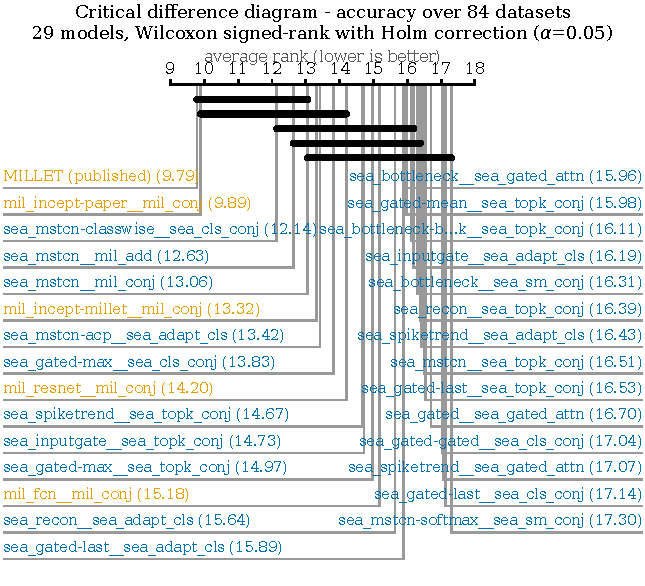
\includegraphics[width=\linewidth]{results/paper_figures/01_main_figures/fig4_critical_difference_accuracy}
  \caption{Critical difference diagram over 84 datasets for the 28 models with a complete sweep. Models are placed by average rank (accuracy), best on the left. A thick horizontal bar joins models whose pairwise differences are not statistically significant under a Wilcoxon signed-rank test with Holm correction at $\alpha$=0.05; models sharing a bar cannot be separated by this evidence. Labels read \texttt{encoder\_\_pooling}, abbreviated, where sea\_ marks a component introduced in this work and mil\_ one reused unchanged from MILLET.}
  \label{fig:fig4_critical_difference_accuracy}
\end{figure}

% Win / tie / loss against MILLET (accuracy)
% Question answered: How often does each model actually beat the published baseline on accuracy?
\begin{figure}[t]
  \centering
  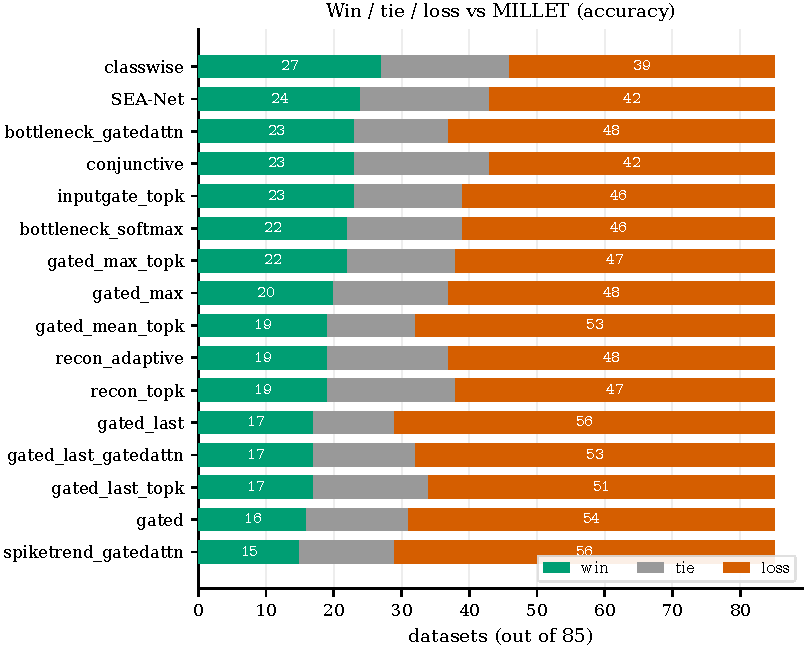
\includegraphics[width=\linewidth]{results/paper_figures/01_main_figures/fig5_win_tie_loss_accuracy}
  \caption{Per-dataset accuracy record of each fully-swept model against the published MILLET results, over the 84 datasets both report. Differences within 0.005 count as ties, since that is below the resolution of these test sets. Sorted by number of wins.}
  \label{fig:fig5_win_tie_loss_accuracy}
\end{figure}

% ===== WebTraffic dataset figures (4 figures) =====

% WebTraffic Accuracy - top 10
% Question answered: Which models explain and classify WebTraffic best on Accuracy?
\begin{figure}[t]
  \centering
  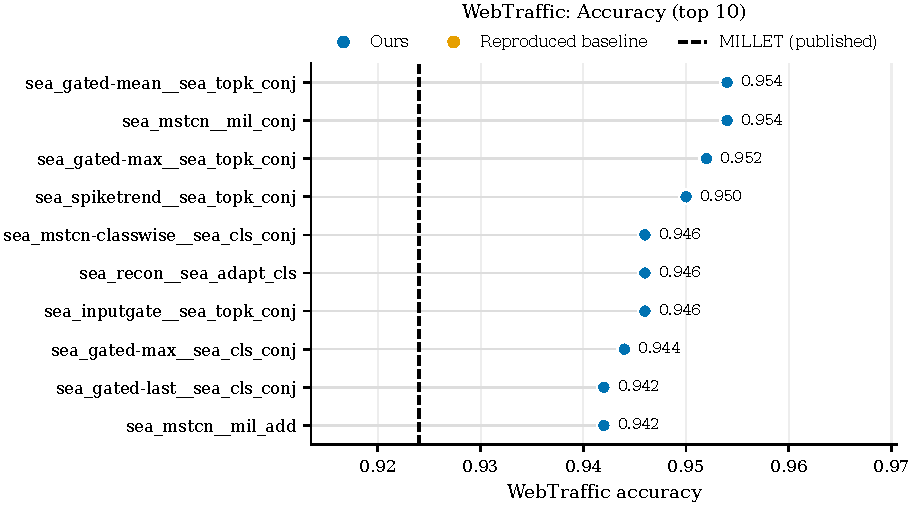
\includegraphics[width=\linewidth]{results/paper_figures/04_web/web_top10_web_acc}
  \caption{WebTraffic accuracy for the 10 best models. WebTraffic is the only dataset with per-timestep ground truth, so it is the only setting where explanation quality can be measured directly rather than estimated. Higher is better.}
  \label{fig:web_top10_web_acc}
\end{figure}

% WebTraffic AOPCR - top 10
% Question answered: Which models explain and classify WebTraffic best on AOPCR?
\begin{figure}[t]
  \centering
  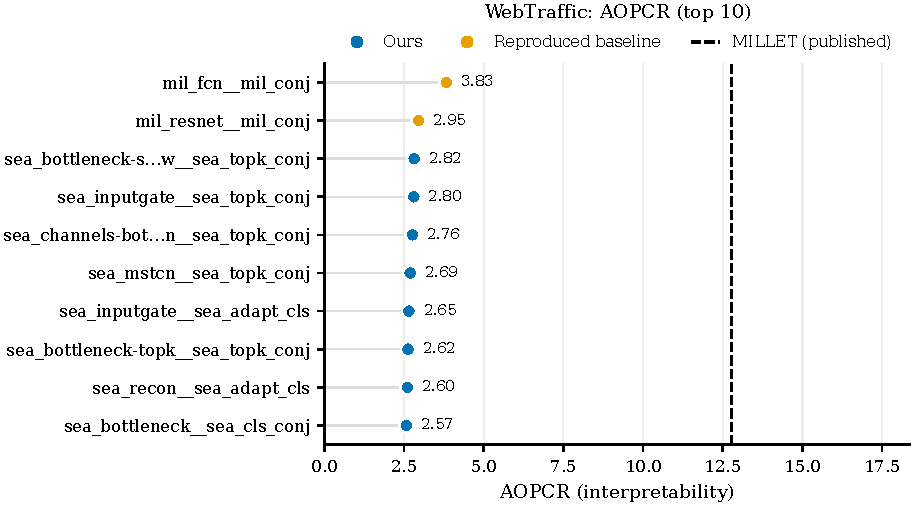
\includegraphics[width=\linewidth]{results/paper_figures/04_web/web_top10_web_aopcr}
  \caption{AOPCR (interpretability) for the 10 best models. WebTraffic is the only dataset with per-timestep ground truth, so it is the only setting where explanation quality can be measured directly rather than estimated. Higher is better.}
  \label{fig:web_top10_web_aopcr}
\end{figure}

% WebTraffic NDCG@n - top 10
% Question answered: Which models explain and classify WebTraffic best on NDCG@n?
\begin{figure}[t]
  \centering
  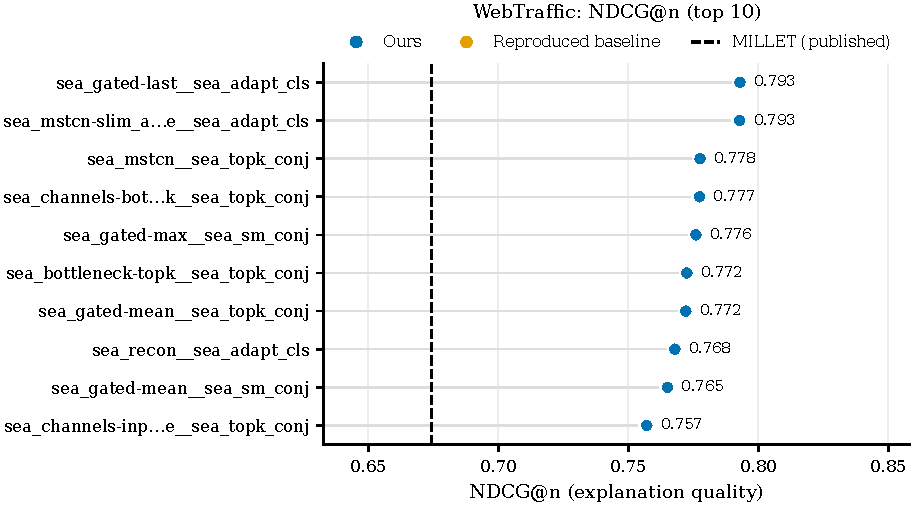
\includegraphics[width=\linewidth]{results/paper_figures/04_web/web_top10_web_ndcg}
  \caption{NDCG@n (explanation quality) for the 10 best models. WebTraffic is the only dataset with per-timestep ground truth, so it is the only setting where explanation quality can be measured directly rather than estimated. Higher is better.}
  \label{fig:web_top10_web_ndcg}
\end{figure}

% WebTraffic Loss - top 10
% Question answered: Which models explain and classify WebTraffic best on Loss?
\begin{figure}[t]
  \centering
  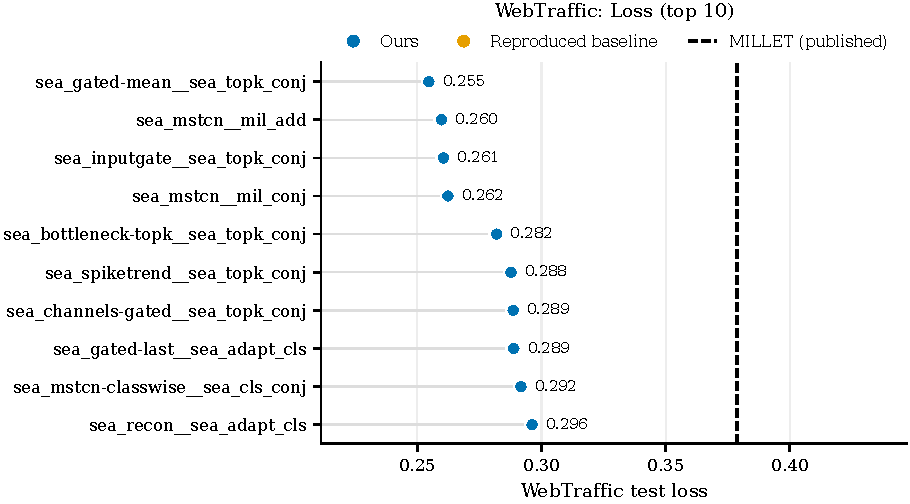
\includegraphics[width=\linewidth]{results/paper_figures/04_web/web_top10_web_loss}
  \caption{WebTraffic test loss for the 10 best models. WebTraffic is the only dataset with per-timestep ground truth, so it is the only setting where explanation quality can be measured directly rather than estimated. Lower is better.}
  \label{fig:web_top10_web_loss}
\end{figure}

% ===== Ablation figures (4 figures) =====

% Accuracy by encoder (pooling head varies within each group)
% Question answered: Which encoder gives the best accuracy, independently of the pooling head?
\begin{figure}[t]
  \centering
  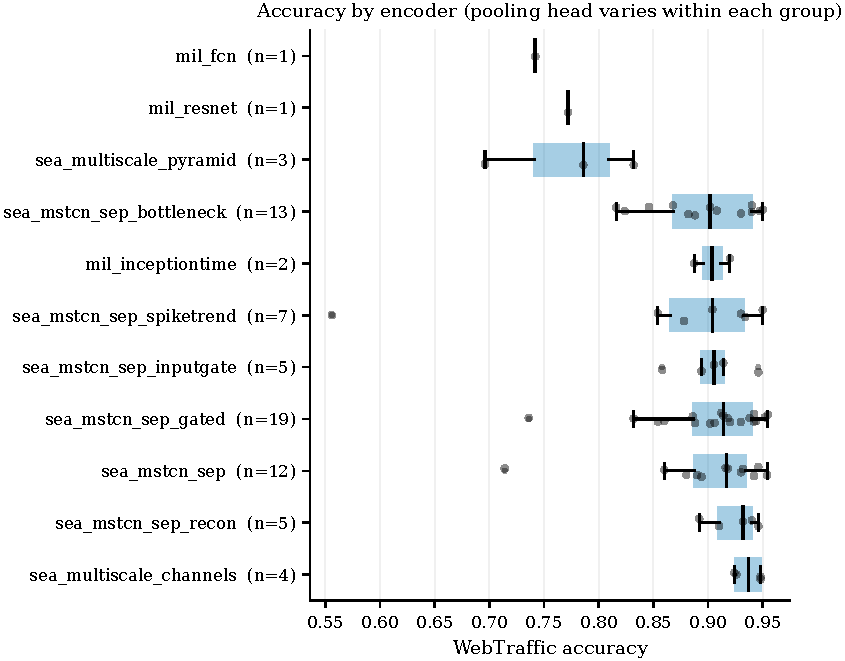
\includegraphics[width=\linewidth]{results/paper_figures/02_ablation/ablation_encoder}
  \caption{WebTraffic accuracy grouped by encoder. Each box covers every model built on that encoder, so the spread shows how much the choice of pooling head still matters once the encoder is fixed. Dots are individual models; n is the group size.}
  \label{fig:ablation_encoder}
\end{figure}

% Accuracy by pooling head (encoder varies within each group)
% Question answered: Which pooling head gives the best accuracy, independently of the encoder?
\begin{figure}[t]
  \centering
  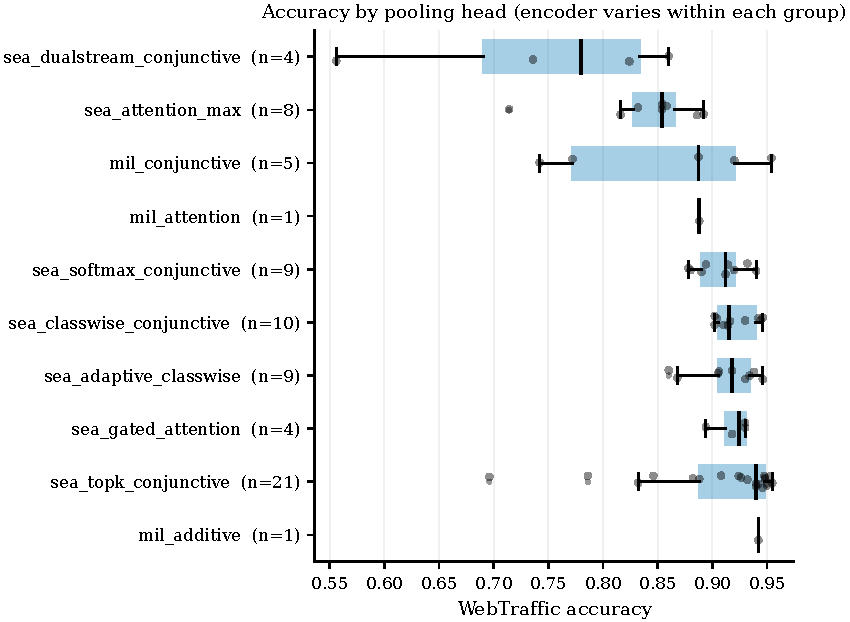
\includegraphics[width=\linewidth]{results/paper_figures/02_ablation/ablation_pooling}
  \caption{WebTraffic accuracy grouped by MIL pooling head. Heads prefixed mil\_ are reused unchanged from MILLET; heads prefixed sea\_ are proposed in this work. Dots are individual models; n is the group size.}
  \label{fig:ablation_pooling}
\end{figure}

% Accuracy by how much of the model is new
% Question answered: Do models with more new components actually perform better?
\begin{figure}[t]
  \centering
  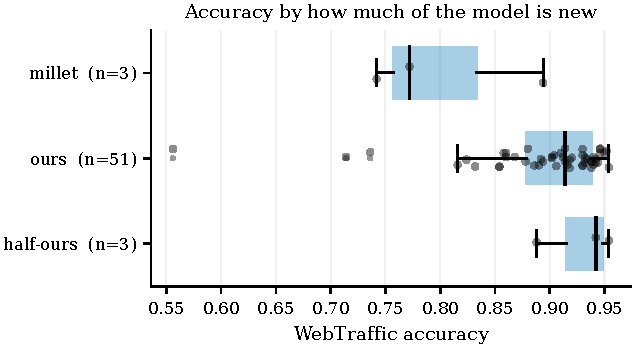
\includegraphics[width=\linewidth]{results/paper_figures/02_ablation/ablation_origin}
  \caption{WebTraffic accuracy grouped by provenance: millet (both halves reproduced from the paper), half-ours (one new half), ours (both halves new). This isolates whether the gains come from the new components or from the shared training recipe.}
  \label{fig:ablation_origin}
\end{figure}

% Encoder x pooling accuracy grid
% Question answered: Which encoder and pooling-head COMBINATION works best, rather than which part?
\begin{figure}[t]
  \centering
  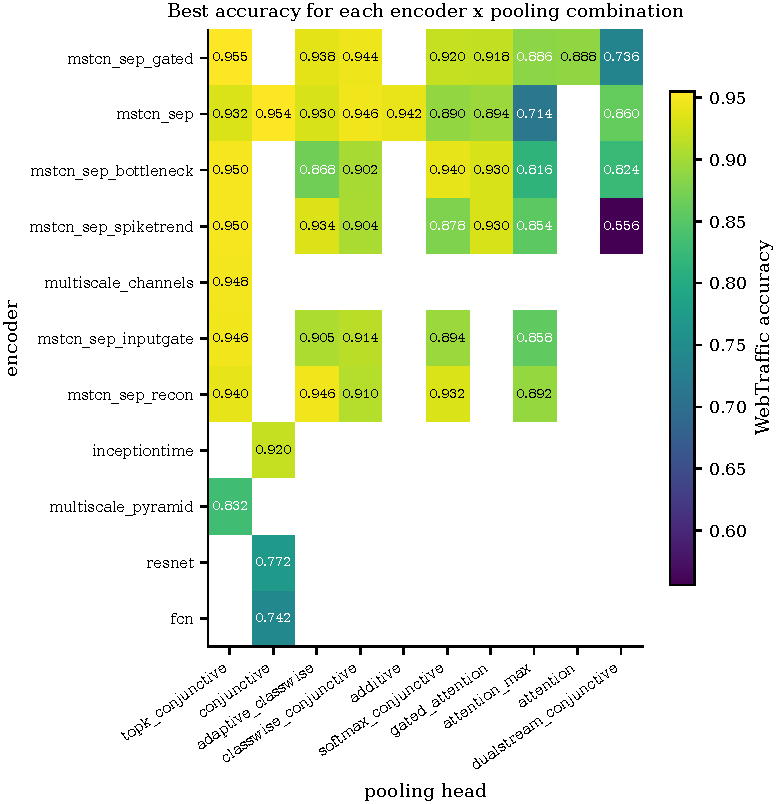
\includegraphics[width=\linewidth]{results/paper_figures/02_ablation/ablation_encoder_pooling_grid}
  \caption{Best WebTraffic accuracy achieved by each encoder and pooling-head combination. Blank cells were never trained. Rows and columns are sorted by their best value, so strong components appear top-left. Prefixes are dropped from the labels for space: all encoders and heads named here are sea\_ (ours) except those marked otherwise in the text.}
  \label{fig:ablation_encoder_pooling_grid}
\end{figure}

% ===== Statistical analysis figures (6 figures) =====

% Accuracy vs AOPCR
% Question answered: Does improving accuracy cost aopcr?
\begin{figure}[t]
  \centering
  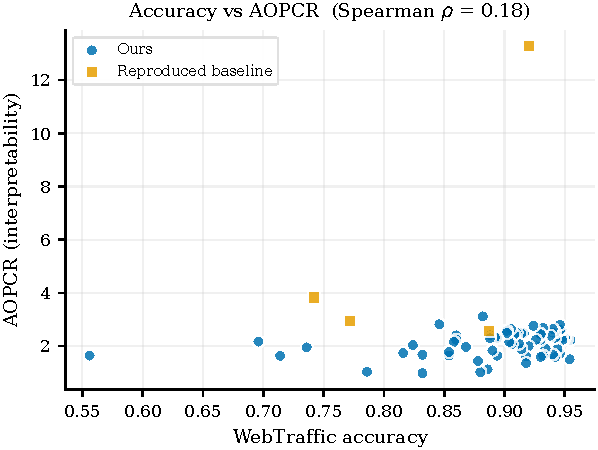
\includegraphics[width=\linewidth]{results/paper_figures/05_statistics/tradeoff_web_acc_vs_web_aopcr}
  \caption{WebTraffic accuracy against AOPCR (interpretability) for every evaluated model. Spearman rank correlation is 0.20: a value near zero means the two objectives are largely independent, so gains on one do not have to be paid for on the other.}
  \label{fig:tradeoff_web_acc_vs_web_aopcr}
\end{figure}

% Accuracy vs NDCG@n
% Question answered: Does improving accuracy cost ndcg@n?
\begin{figure}[t]
  \centering
  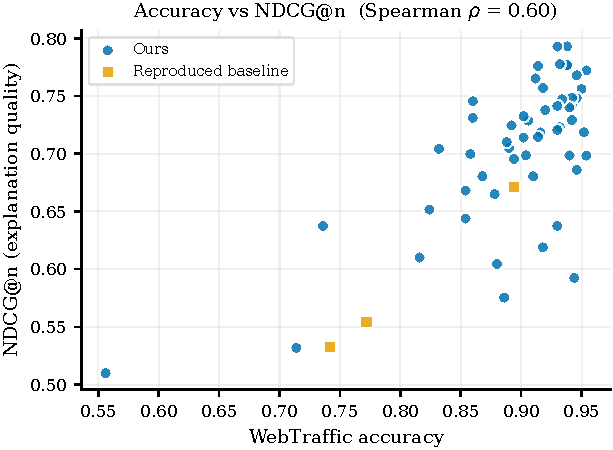
\includegraphics[width=\linewidth]{results/paper_figures/05_statistics/tradeoff_web_acc_vs_web_ndcg}
  \caption{WebTraffic accuracy against NDCG@n (explanation quality) for every evaluated model. Spearman rank correlation is 0.60: a value near zero means the two objectives are largely independent, so gains on one do not have to be paid for on the other.}
  \label{fig:tradeoff_web_acc_vs_web_ndcg}
\end{figure}

% Average rank (accuracy)
% Question answered: Which model is best overall on accuracy, robust to individual datasets?
\begin{figure}[t]
  \centering
  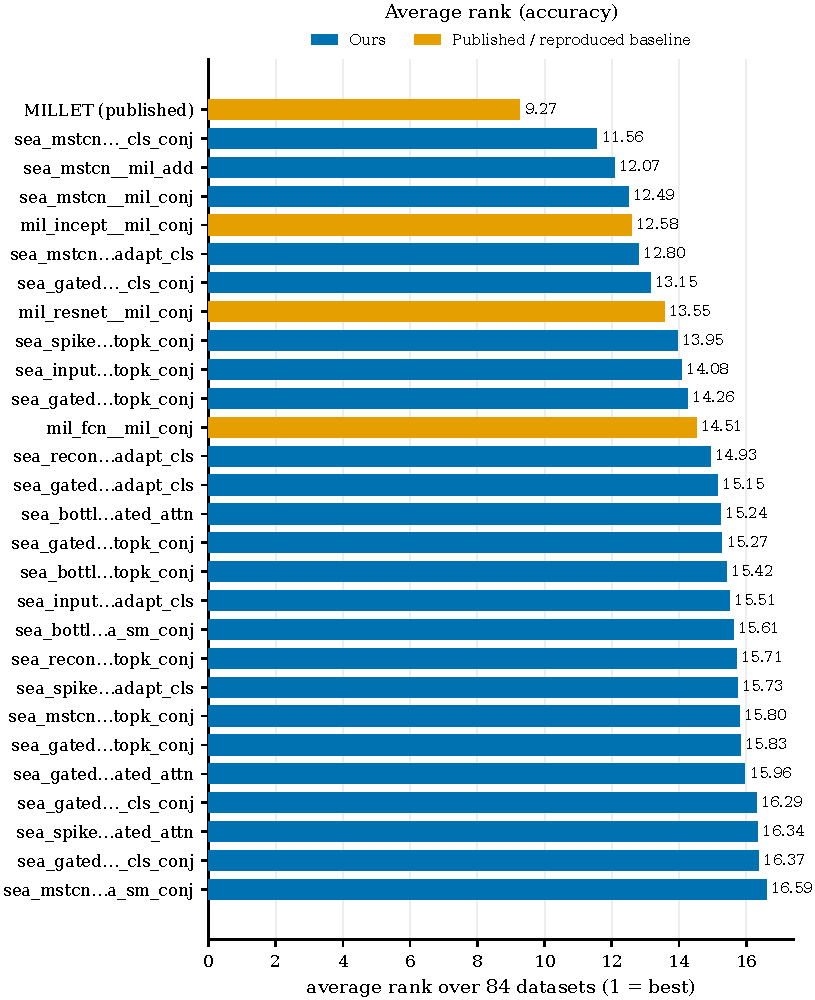
\includegraphics[width=\linewidth]{results/paper_figures/05_statistics/stats_average_rank_accuracy}
  \caption{Average accuracy rank of each fully-swept model over 84 datasets (rank 1 is best on a dataset). Ranking is robust to a single easy dataset in a way that a mean is not.}
  \label{fig:stats_average_rank_accuracy}
\end{figure}

% Average improvement over MILLET (accuracy)
% Question answered: By how much does each model improve on the baseline in accuracy?
\begin{figure}[t]
  \centering
  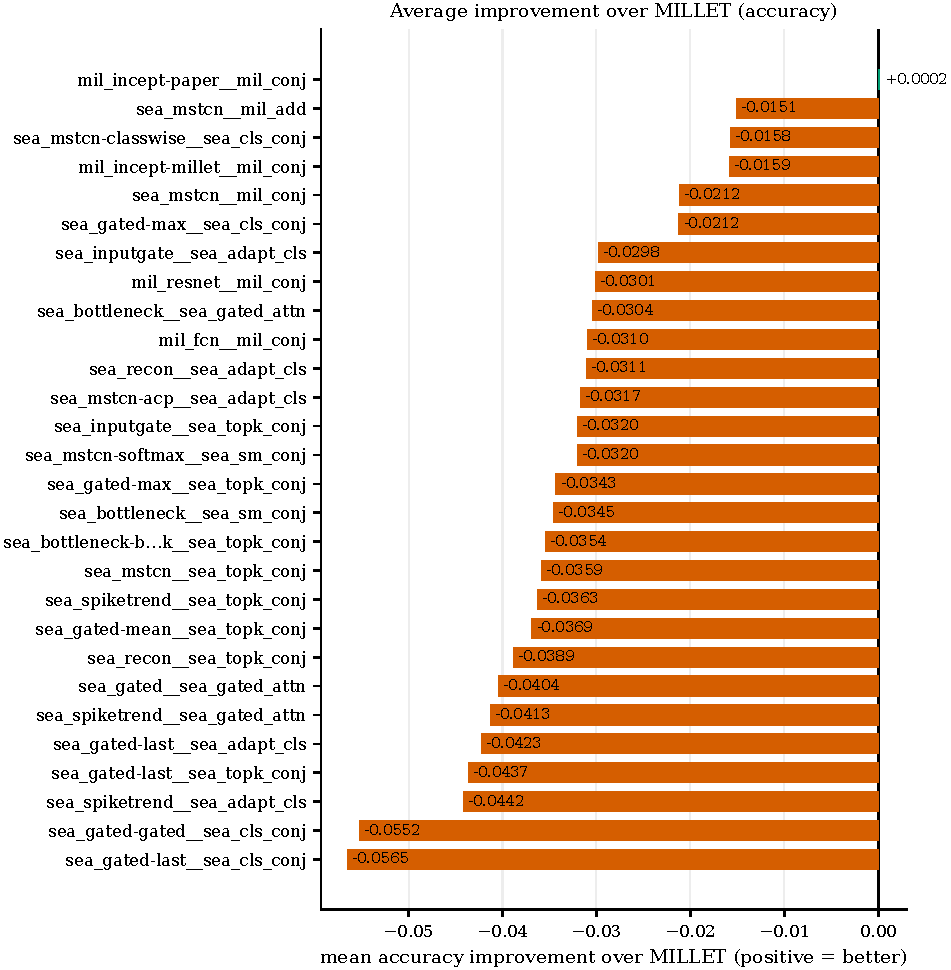
\includegraphics[width=\linewidth]{results/paper_figures/05_statistics/stats_improvement_over_millet_accuracy}
  \caption{Mean per-dataset accuracy difference against the published MILLET results. Green bars improve on the baseline, red bars fall short. Read together with the win/tie/loss figure: this shows the size of the gap, that one shows how often it goes each way.}
  \label{fig:stats_improvement_over_millet_accuracy}
\end{figure}

% Pairwise win matrix (accuracy)
% Question answered: Which models beat which other models directly, rather than on average?
\begin{figure*}[t]
  \centering
  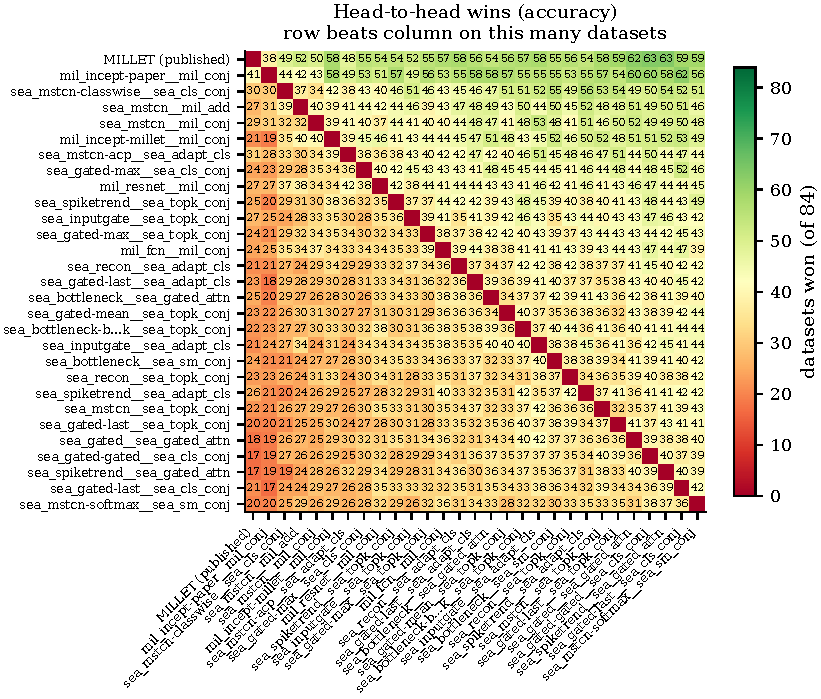
\includegraphics[width=\linewidth]{results/paper_figures/05_statistics/stats_pairwise_wins_accuracy}
  \caption{Head-to-head accuracy record over 84 datasets: the cell in row i and column j counts the datasets on which model i beats model j. Models are ordered by average rank, so a well-ordered matrix is green above the diagonal.}
  \label{fig:stats_pairwise_wins_accuracy}
\end{figure*}

% Metric correlation
% Question answered: Are our metrics measuring different things, or repeating each other?
\begin{figure}[t]
  \centering
  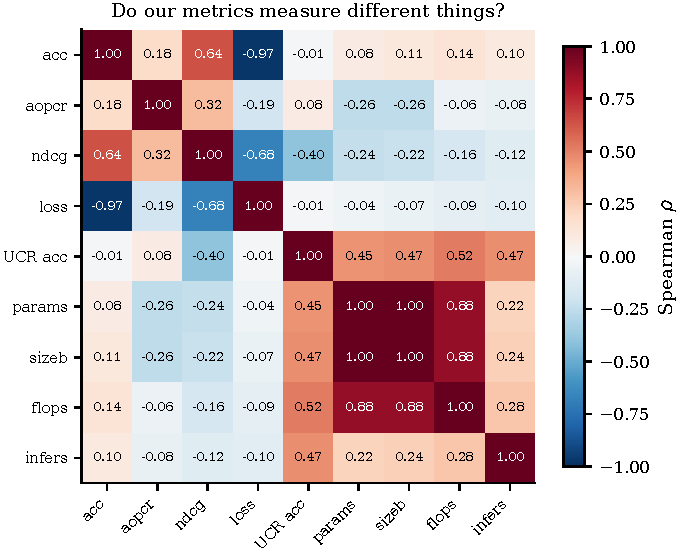
\includegraphics[width=\linewidth]{results/paper_figures/05_statistics/stats_metric_correlation}
  \caption{Spearman rank correlation between every reported metric across all evaluated models. Rank correlation is used because what matters is whether two metrics order the models the same way. Values near zero identify genuinely independent axes, which is why they are reported separately rather than combined into one score.}
  \label{fig:stats_metric_correlation}
\end{figure}

% ===== Appendix figures (23 figures) =====

% Benchmark band 3: remaining models (Accuracy)
% Question answered: Which models are the remaining on Accuracy?
\begin{figure}[t]
  \centering
  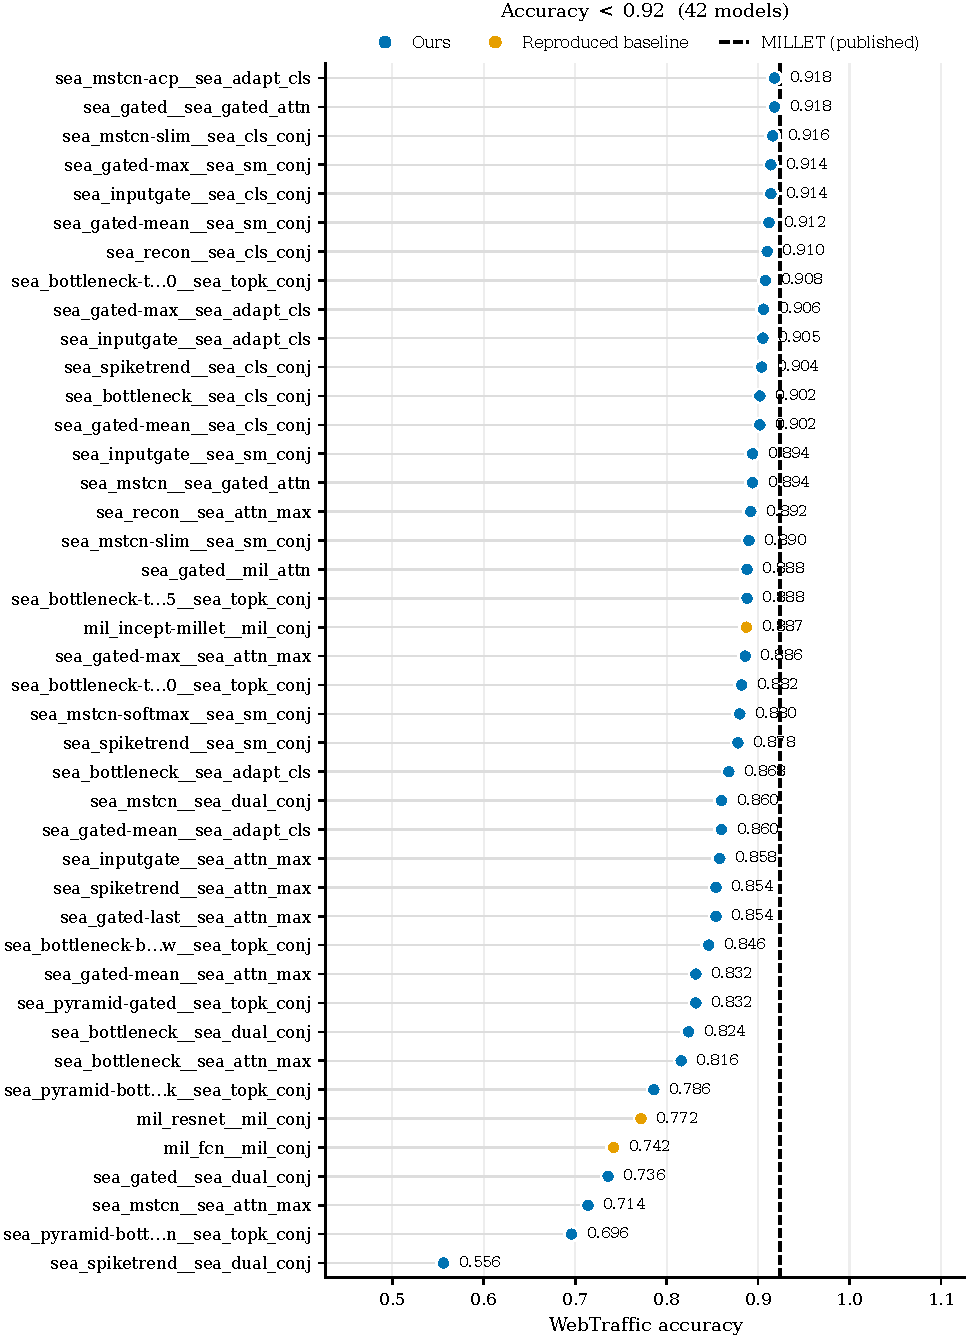
\includegraphics[width=\linewidth]{results/paper_figures/03_appendix/fig3_benchmark_remaining_web_acc}
  \caption{Accuracy of the remaining models on WebTraffic (34 models, Accuracy $<$ 0.93). Bars are sorted best-first; blue marks models proposed in this work and orange our reproduction of the published backbones. Labels read \texttt{encoder\_\_pooling}, abbreviated, where sea\_ marks a component introduced here and mil\_ one reused unchanged from MILLET. The dashed line is the accuracy reported in the MILLET paper. Bands are disjoint, so each model appears in exactly one of Figures 1--3.}
  \label{fig:fig3_benchmark_remaining_web_acc}
\end{figure}

% WebTraffic Accuracy - every model
% Question answered: How does the complete field of models compare on WebTraffic Accuracy?
\begin{figure}[t]
  \centering
  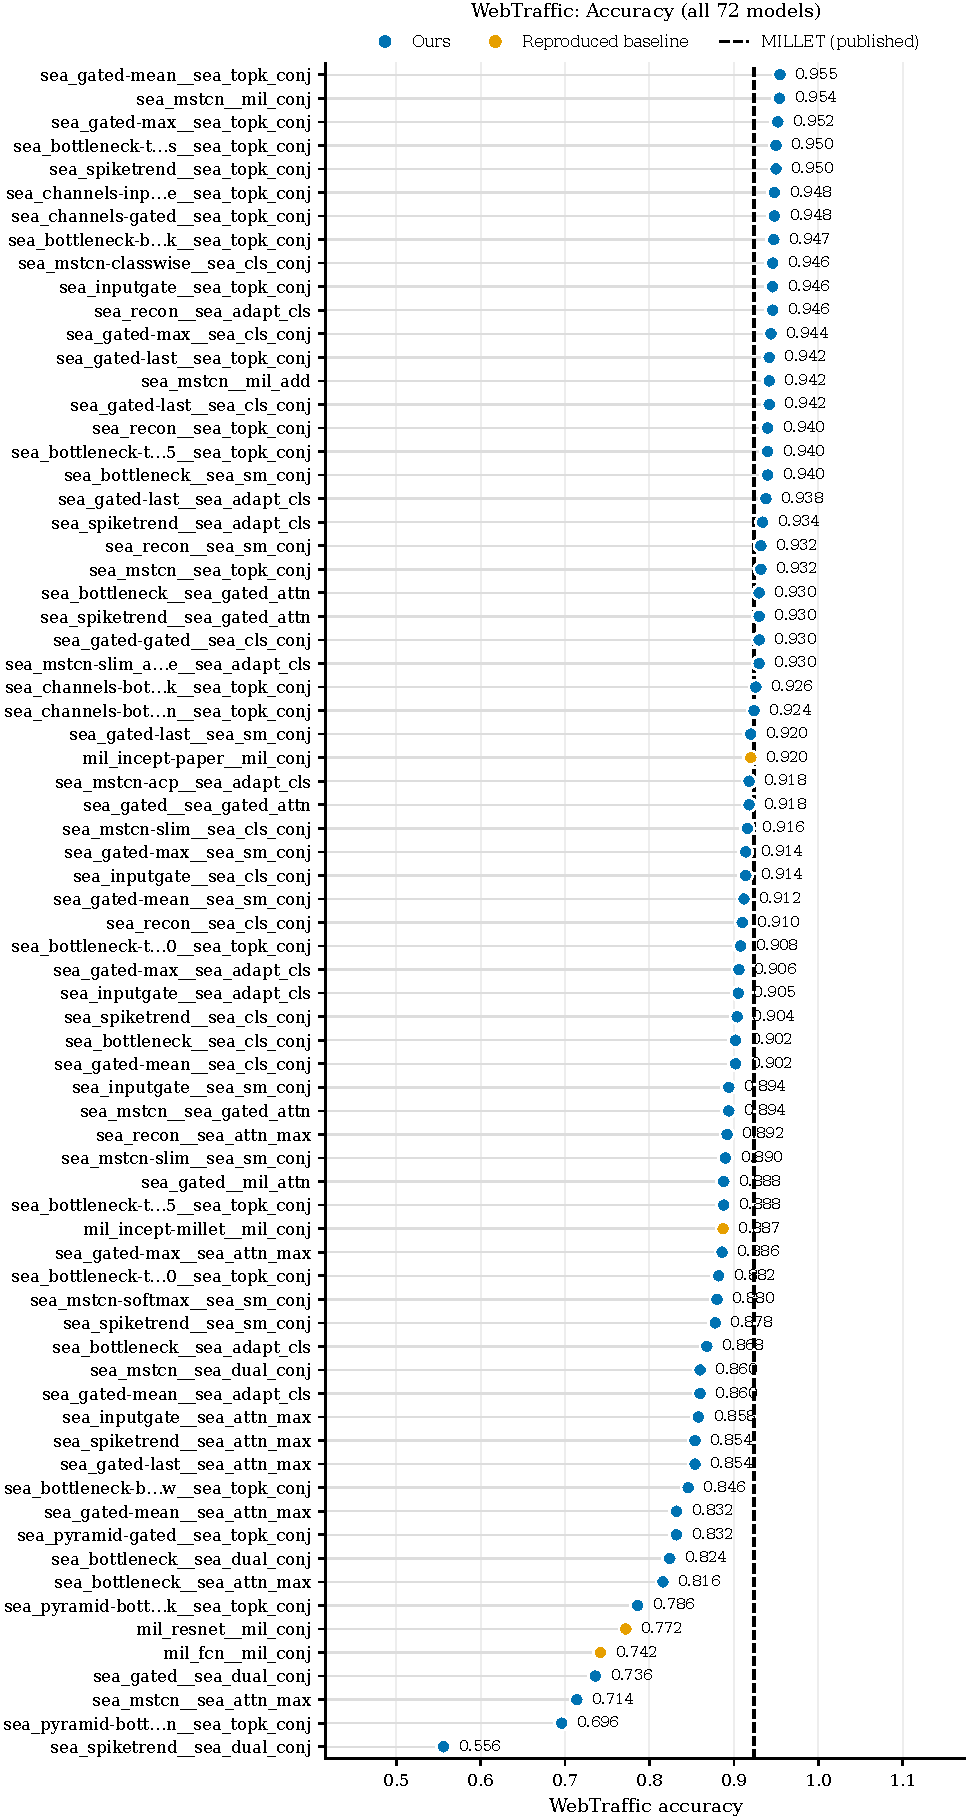
\includegraphics[width=\linewidth]{results/paper_figures/03_appendix/appendix_web_all_web_acc}
  \caption{WebTraffic accuracy for all 57 evaluated models, sorted best-first. The main-paper version of this figure shows only the top 10.}
  \label{fig:appendix_web_all_web_acc}
\end{figure}

% WebTraffic AOPCR - every model
% Question answered: How does the complete field of models compare on WebTraffic AOPCR?
\begin{figure}[t]
  \centering
  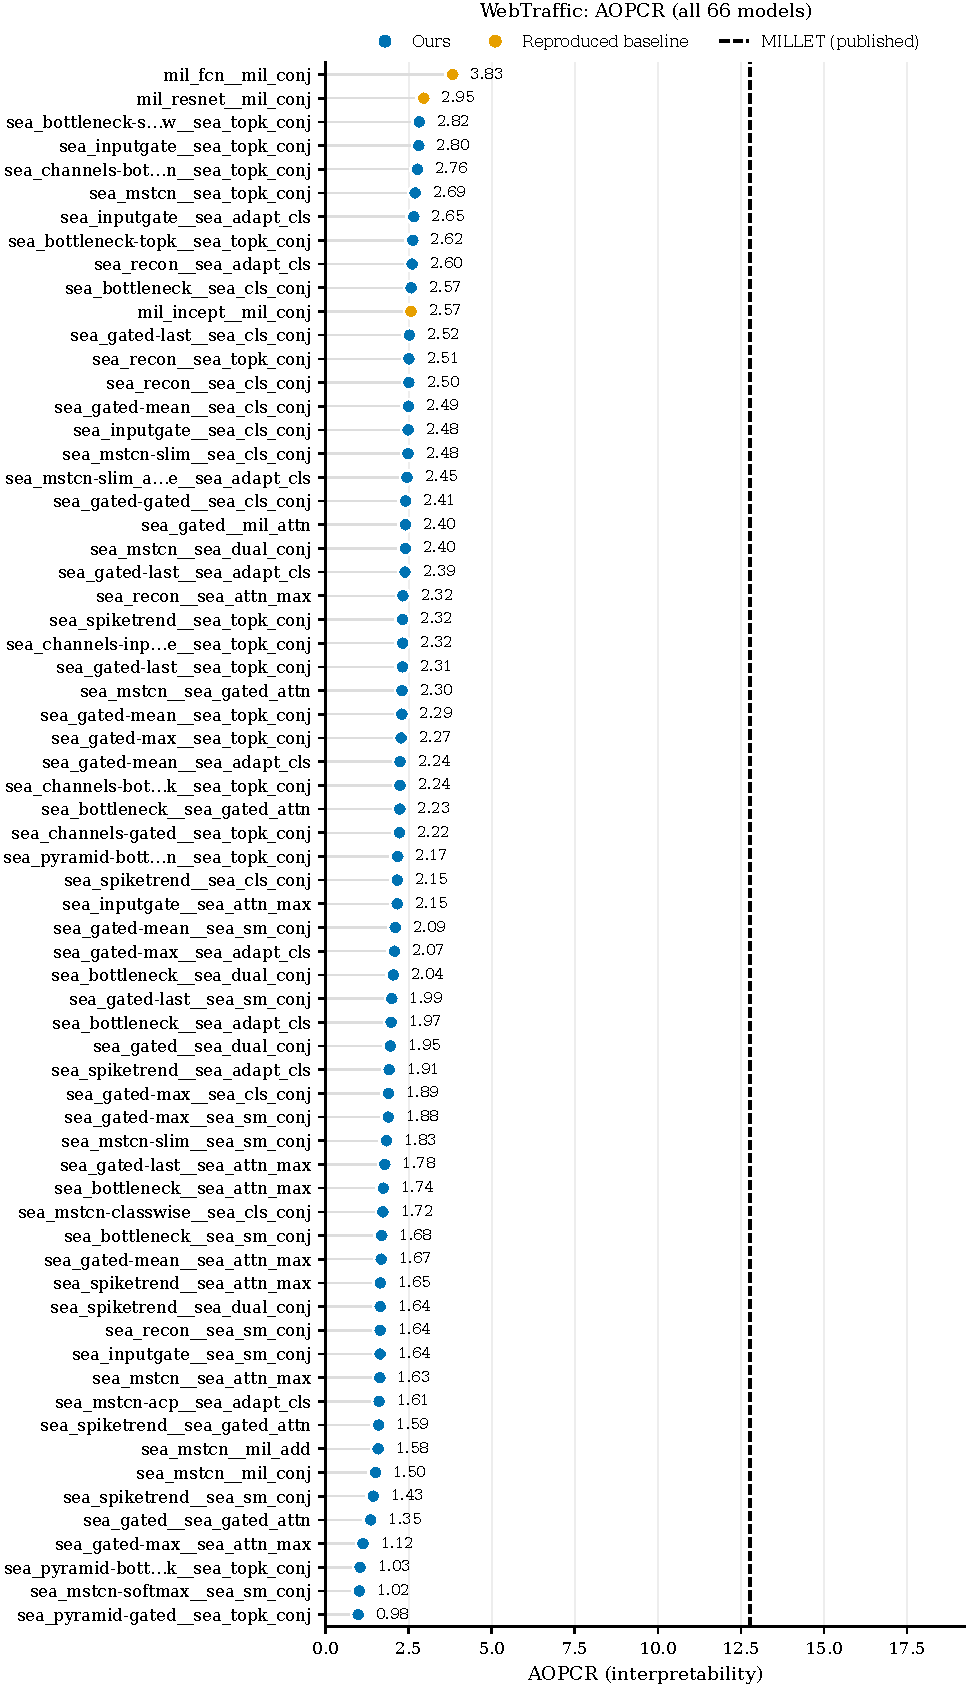
\includegraphics[width=\linewidth]{results/paper_figures/03_appendix/appendix_web_all_web_aopcr}
  \caption{AOPCR (interpretability) for all 57 evaluated models, sorted best-first. The main-paper version of this figure shows only the top 10.}
  \label{fig:appendix_web_all_web_aopcr}
\end{figure}

% WebTraffic NDCG@n - every model
% Question answered: How does the complete field of models compare on WebTraffic NDCG@n?
\begin{figure}[t]
  \centering
  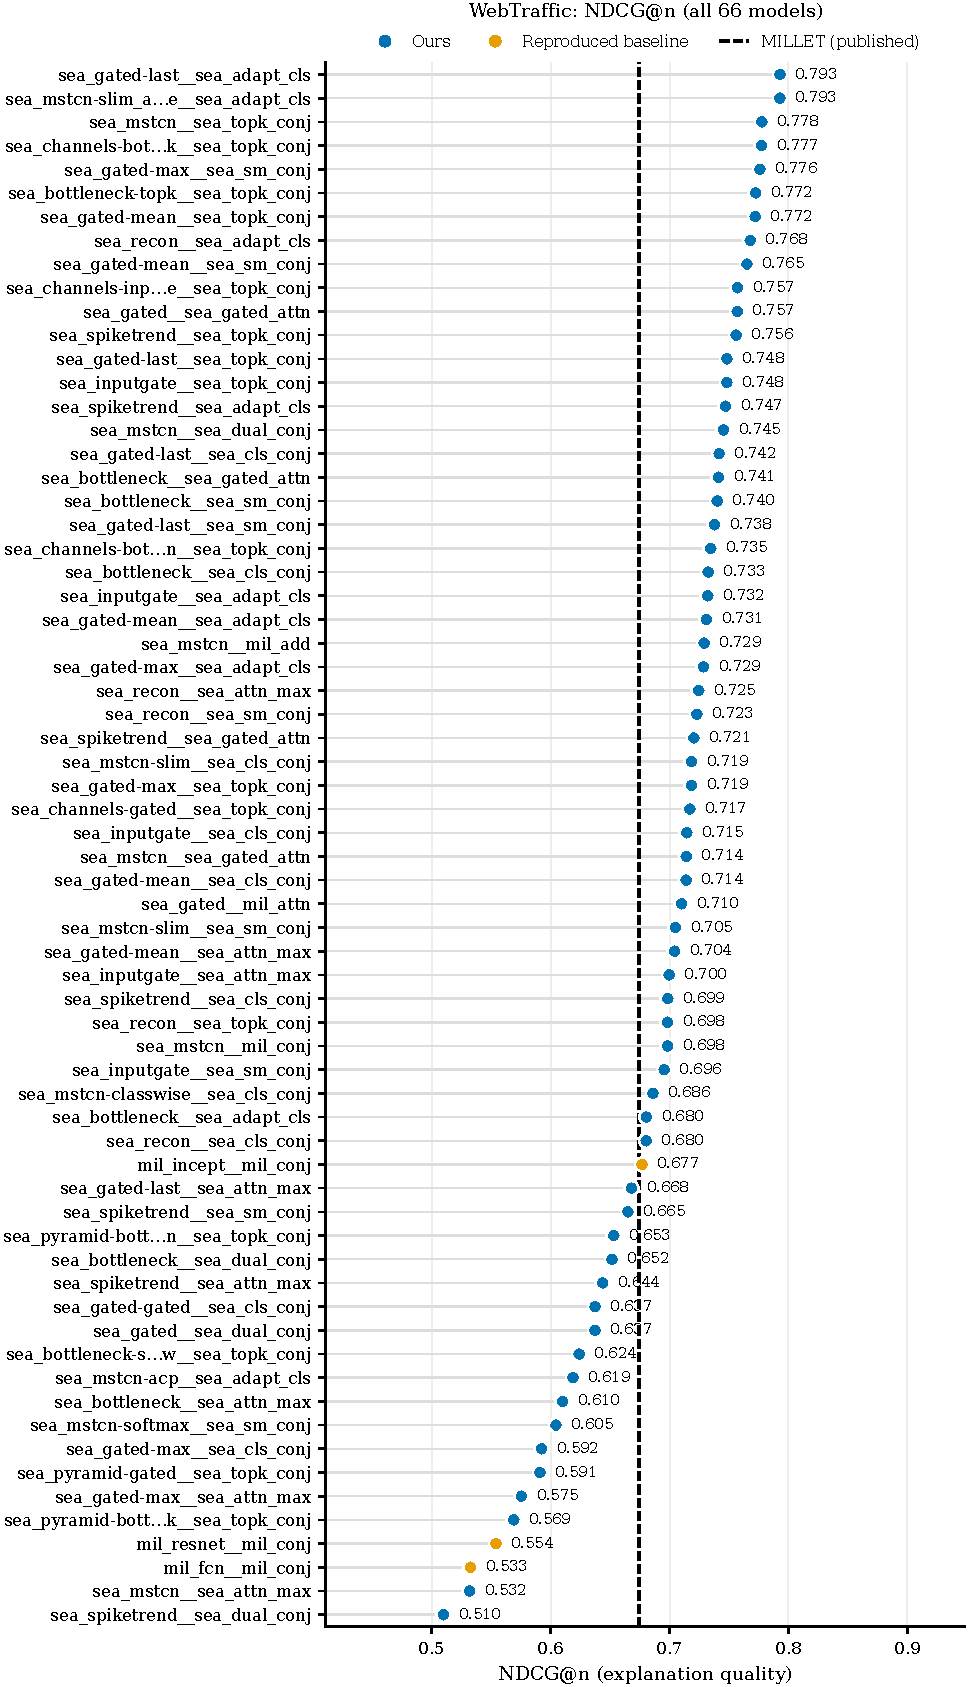
\includegraphics[width=\linewidth]{results/paper_figures/03_appendix/appendix_web_all_web_ndcg}
  \caption{NDCG@n (explanation quality) for all 57 evaluated models, sorted best-first. The main-paper version of this figure shows only the top 10.}
  \label{fig:appendix_web_all_web_ndcg}
\end{figure}

% WebTraffic Loss - every model
% Question answered: How does the complete field of models compare on WebTraffic Loss?
\begin{figure}[t]
  \centering
  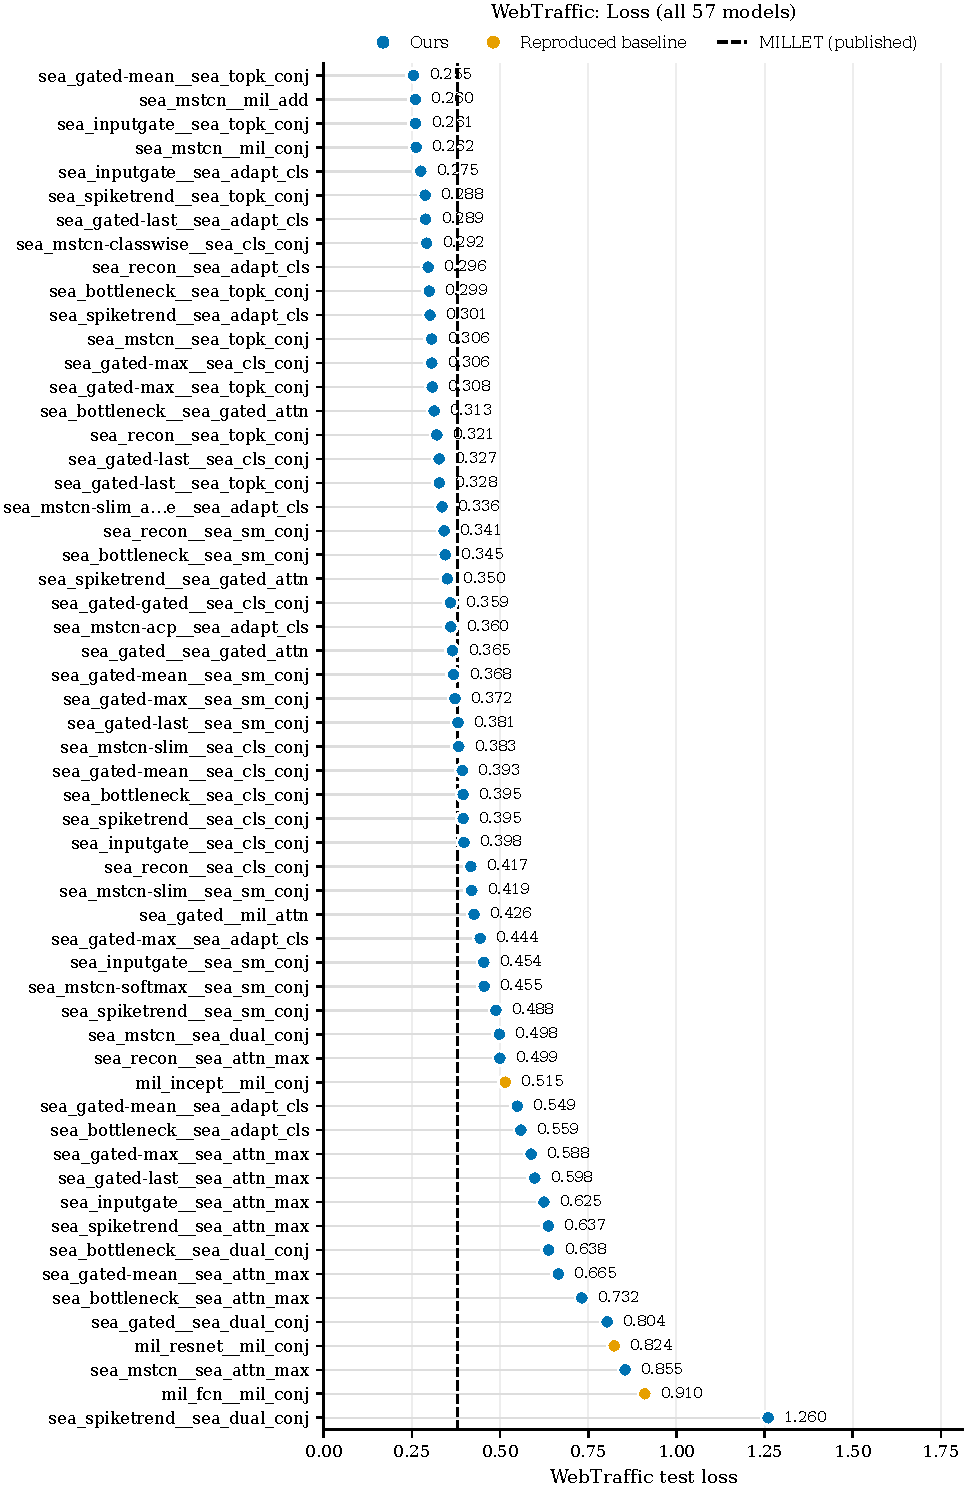
\includegraphics[width=\linewidth]{results/paper_figures/03_appendix/appendix_web_all_web_loss}
  \caption{WebTraffic test loss for all 57 evaluated models, sorted best-first. The main-paper version of this figure shows only the top 10.}
  \label{fig:appendix_web_all_web_loss}
\end{figure}

% Accuracy vs Model size (Pareto)
% Question answered: Does a smaller model stay competitive once model size is taken into account?
\begin{figure}[t]
  \centering
  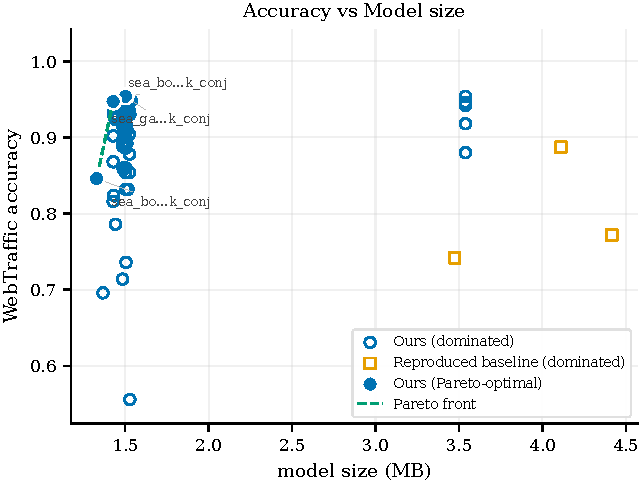
\includegraphics[width=\linewidth]{results/paper_figures/03_appendix/pareto_web_acc_vs_size_mb}
  \caption{WebTraffic accuracy against model size (MB). Filled markers joined by the dashed line are Pareto-optimal: no other model is both cheaper and better. Hollow markers are dominated and therefore never the right choice. Only Pareto-optimal models are labelled.}
  \label{fig:pareto_web_acc_vs_size_mb}
\end{figure}

% Accuracy vs FLOPs (Pareto)
% Question answered: Does a smaller model stay competitive once flops is taken into account?
\begin{figure}[t]
  \centering
  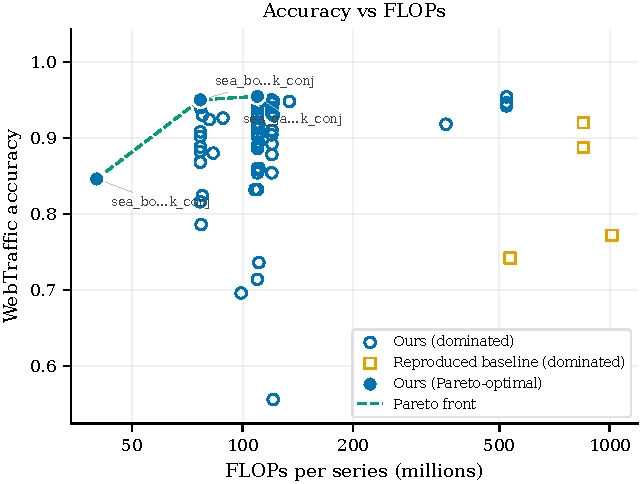
\includegraphics[width=\linewidth]{results/paper_figures/03_appendix/pareto_web_acc_vs_flops_m}
  \caption{WebTraffic accuracy against FLOPs per series (millions). Filled markers joined by the dashed line are Pareto-optimal: no other model is both cheaper and better. Hollow markers are dominated and therefore never the right choice. Only Pareto-optimal models are labelled.}
  \label{fig:pareto_web_acc_vs_flops_m}
\end{figure}

% Accuracy vs Inference time (Pareto)
% Question answered: Does a smaller model stay competitive once inference time is taken into account?
\begin{figure}[t]
  \centering
  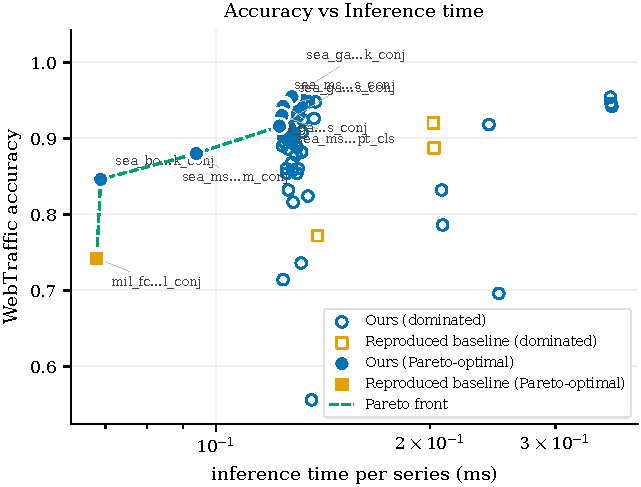
\includegraphics[width=\linewidth]{results/paper_figures/03_appendix/pareto_web_acc_vs_infer_ms}
  \caption{WebTraffic accuracy against inference time per series (ms). Filled markers joined by the dashed line are Pareto-optimal: no other model is both cheaper and better. Hollow markers are dominated and therefore never the right choice. Only Pareto-optimal models are labelled.}
  \label{fig:pareto_web_acc_vs_infer_ms}
\end{figure}

% Accuracy vs GPU memory (Pareto)
% Question answered: Does a smaller model stay competitive once gpu memory is taken into account?
\begin{figure}[t]
  \centering
  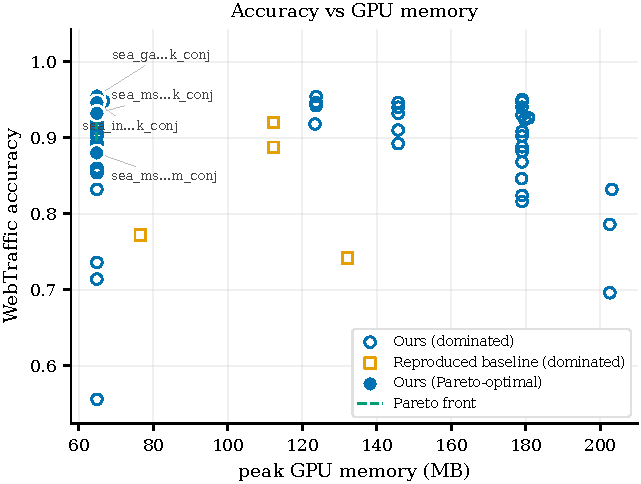
\includegraphics[width=\linewidth]{results/paper_figures/03_appendix/pareto_web_acc_vs_peak_mem_mb}
  \caption{WebTraffic accuracy against peak GPU memory (MB). Filled markers joined by the dashed line are Pareto-optimal: no other model is both cheaper and better. Hollow markers are dominated and therefore never the right choice. Only Pareto-optimal models are labelled.}
  \label{fig:pareto_web_acc_vs_peak_mem_mb}
\end{figure}

% Top-3 models across all metrics
% Question answered: Which of the top-3 models is preferable once every metric is considered?
\begin{figure*}[t]
  \centering
  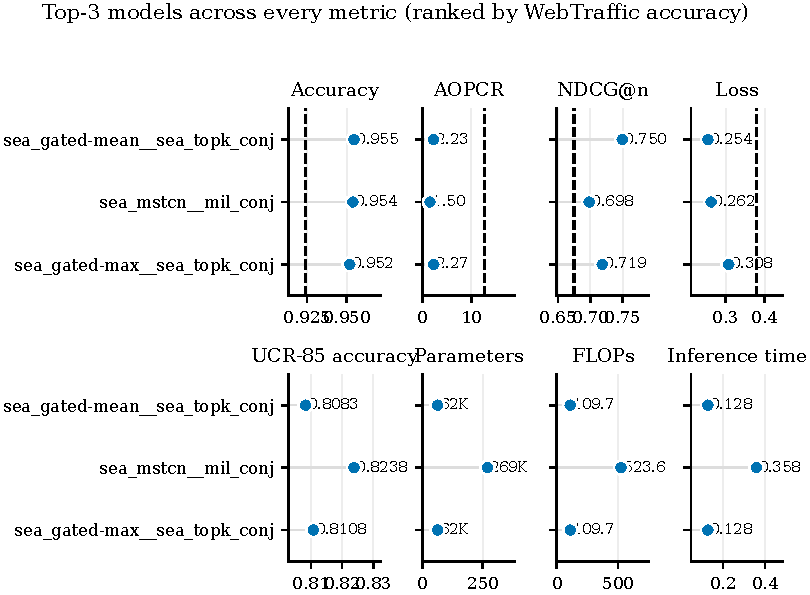
\includegraphics[width=\linewidth]{results/paper_figures/03_appendix/topk3_multimetric}
  \caption{The top-3 models, ranked by WebTraffic accuracy, compared on every available metric. Panels share the same model order, so a single model can be followed across quality (accuracy, AOPCR, NDCG, loss) and cost (parameters, FLOPs, latency). Blue marks models proposed in this work.}
  \label{fig:topk3_multimetric}
\end{figure*}

% Top-5 models - Accuracy
% Question answered: How do the top-5 models compare on Accuracy alone?
\begin{figure*}[t]
  \centering
  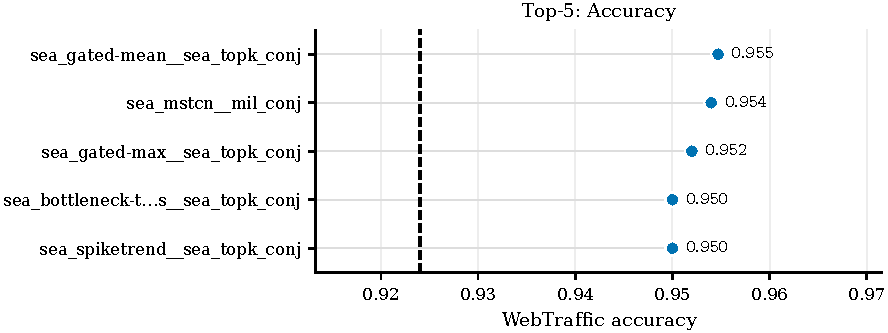
\includegraphics[width=\linewidth]{results/paper_figures/03_appendix/topk5_web_acc}
  \caption{Accuracy of the top-5 models (ranked by WebTraffic accuracy). Higher is better.}
  \label{fig:topk5_web_acc}
\end{figure*}

% Top-5 models - AOPCR
% Question answered: How do the top-5 models compare on AOPCR alone?
\begin{figure*}[t]
  \centering
  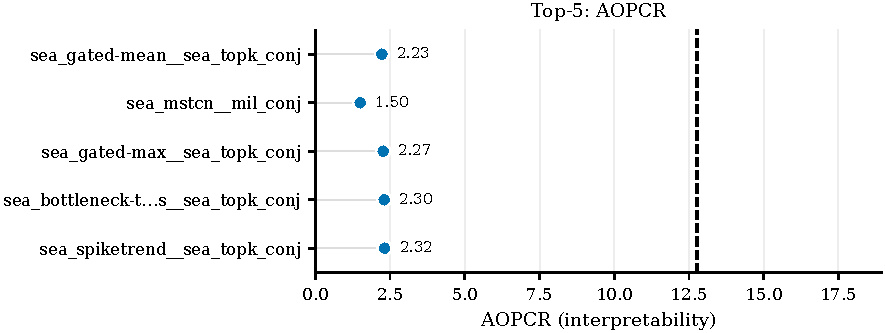
\includegraphics[width=\linewidth]{results/paper_figures/03_appendix/topk5_web_aopcr}
  \caption{AOPCR of the top-5 models (ranked by WebTraffic accuracy). Higher is better.}
  \label{fig:topk5_web_aopcr}
\end{figure*}

% Top-5 models - NDCG@n
% Question answered: How do the top-5 models compare on NDCG@n alone?
\begin{figure*}[t]
  \centering
  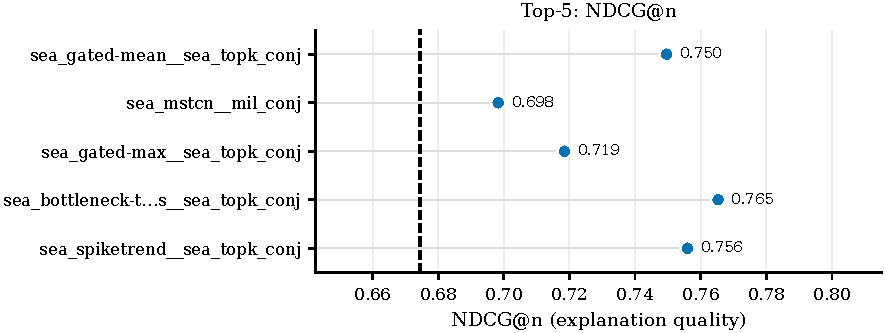
\includegraphics[width=\linewidth]{results/paper_figures/03_appendix/topk5_web_ndcg}
  \caption{NDCG@n of the top-5 models (ranked by WebTraffic accuracy). Higher is better.}
  \label{fig:topk5_web_ndcg}
\end{figure*}

% Top-5 models - Loss
% Question answered: How do the top-5 models compare on Loss alone?
\begin{figure*}[t]
  \centering
  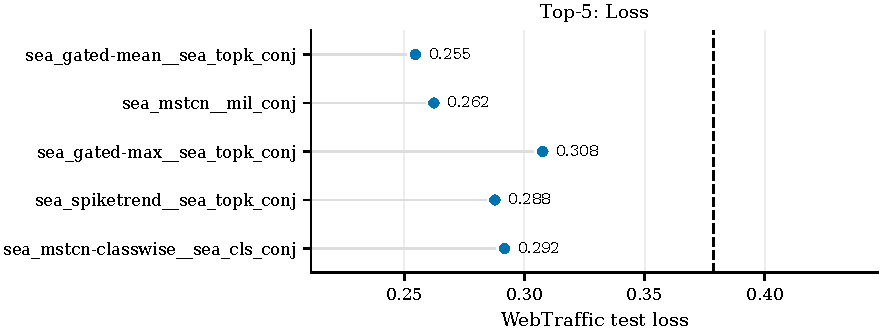
\includegraphics[width=\linewidth]{results/paper_figures/03_appendix/topk5_web_loss}
  \caption{Loss of the top-5 models (ranked by WebTraffic accuracy). Lower is better.}
  \label{fig:topk5_web_loss}
\end{figure*}

% Top-5 models - UCR-85 accuracy
% Question answered: How do the top-5 models compare on UCR-85 accuracy alone?
\begin{figure*}[t]
  \centering
  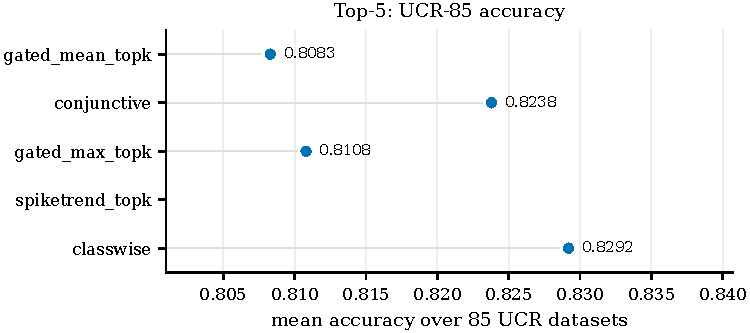
\includegraphics[width=\linewidth]{results/paper_figures/03_appendix/topk5_ucr85_acc}
  \caption{UCR-85 accuracy of the top-5 models (ranked by WebTraffic accuracy). Higher is better.}
  \label{fig:topk5_ucr85_acc}
\end{figure*}

% Top-5 models - Parameters
% Question answered: How do the top-5 models compare on Parameters alone?
\begin{figure*}[t]
  \centering
  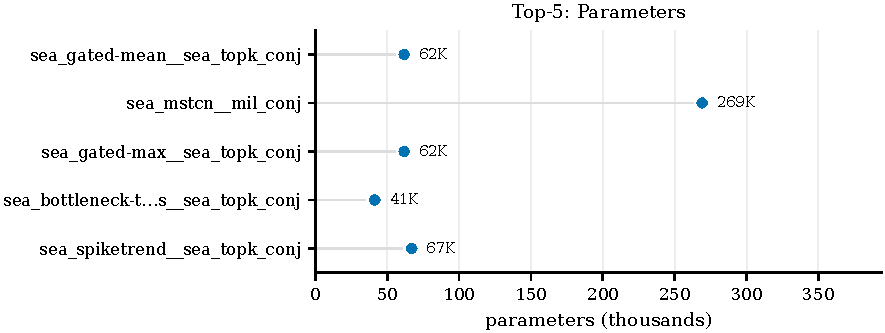
\includegraphics[width=\linewidth]{results/paper_figures/03_appendix/topk5_params}
  \caption{Parameters of the top-5 models (ranked by WebTraffic accuracy). Lower is better.}
  \label{fig:topk5_params}
\end{figure*}

% Top-5 models - Model size
% Question answered: How do the top-5 models compare on Model size alone?
\begin{figure*}[t]
  \centering
  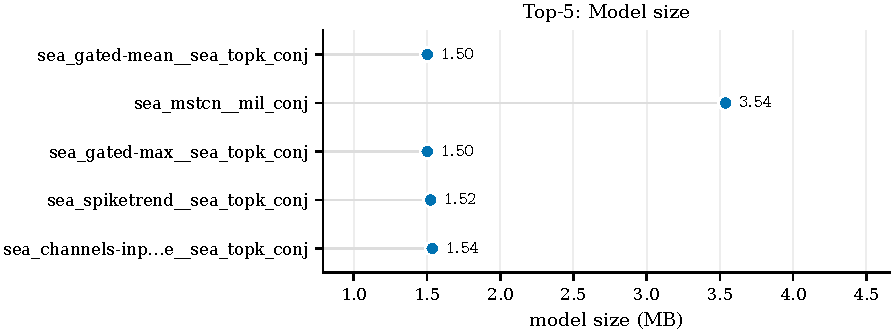
\includegraphics[width=\linewidth]{results/paper_figures/03_appendix/topk5_size_mb}
  \caption{Model size of the top-5 models (ranked by WebTraffic accuracy). Lower is better.}
  \label{fig:topk5_size_mb}
\end{figure*}

% Top-5 models - FLOPs
% Question answered: How do the top-5 models compare on FLOPs alone?
\begin{figure*}[t]
  \centering
  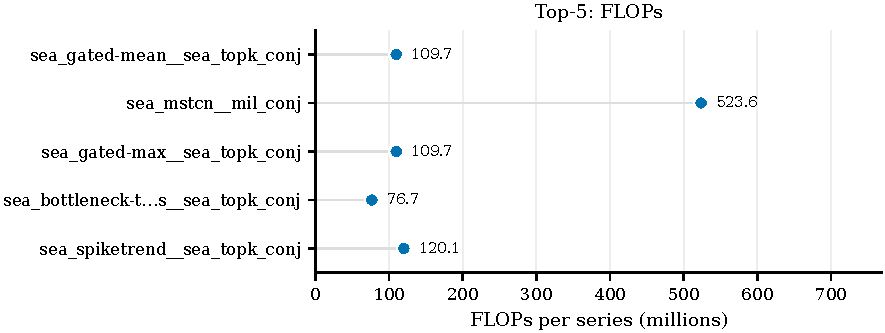
\includegraphics[width=\linewidth]{results/paper_figures/03_appendix/topk5_flops_m}
  \caption{FLOPs of the top-5 models (ranked by WebTraffic accuracy). Lower is better.}
  \label{fig:topk5_flops_m}
\end{figure*}

% Top-5 models - Inference time
% Question answered: How do the top-5 models compare on Inference time alone?
\begin{figure*}[t]
  \centering
  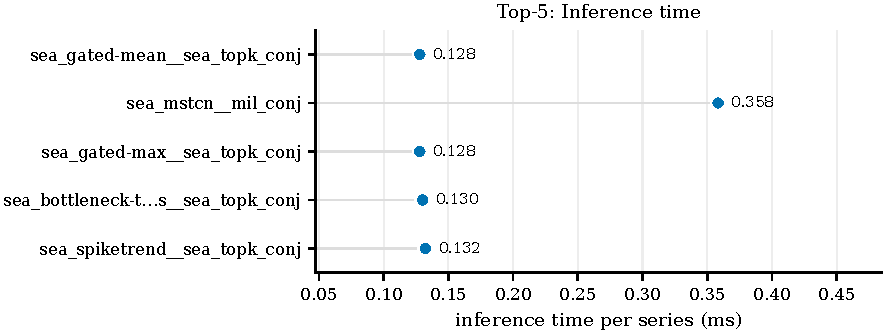
\includegraphics[width=\linewidth]{results/paper_figures/03_appendix/topk5_infer_ms}
  \caption{Inference time of the top-5 models (ranked by WebTraffic accuracy). Lower is better.}
  \label{fig:topk5_infer_ms}
\end{figure*}

% Top-5 models - GPU memory
% Question answered: How do the top-5 models compare on GPU memory alone?
\begin{figure*}[t]
  \centering
  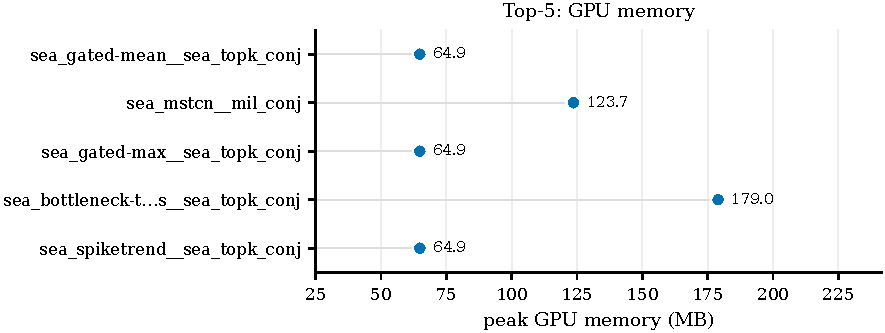
\includegraphics[width=\linewidth]{results/paper_figures/03_appendix/topk5_peak_mem_mb}
  \caption{GPU memory of the top-5 models (ranked by WebTraffic accuracy). Lower is better.}
  \label{fig:topk5_peak_mem_mb}
\end{figure*}

% Top-10 models across all metrics
% Question answered: Which of the top-10 models is preferable once every metric is considered?
\begin{figure*}[t]
  \centering
  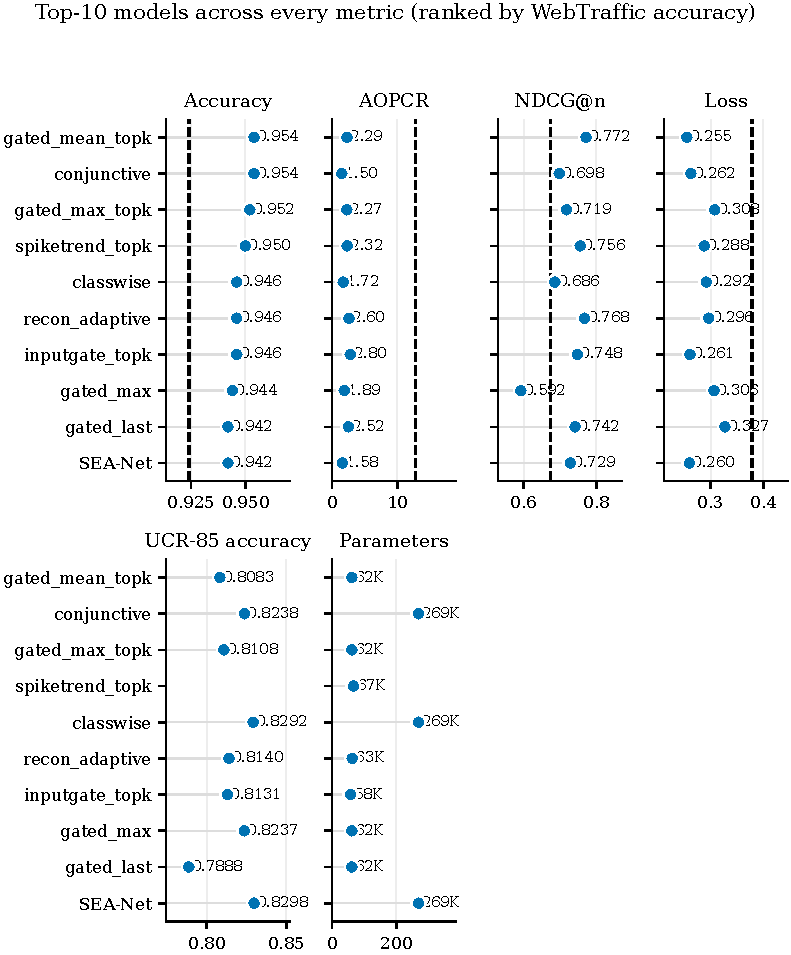
\includegraphics[width=\linewidth]{results/paper_figures/03_appendix/topk10_multimetric}
  \caption{The top-10 models, ranked by WebTraffic accuracy, compared on every available metric. Panels share the same model order, so a single model can be followed across quality (accuracy, AOPCR, NDCG, loss) and cost (parameters, FLOPs, latency). Blue marks models proposed in this work.}
  \label{fig:topk10_multimetric}
\end{figure*}

% Dataset x model heatmap (accuracy)
% Question answered: Where do the gains and losses against the baseline actually come from?
\begin{figure*}[t]
  \centering
  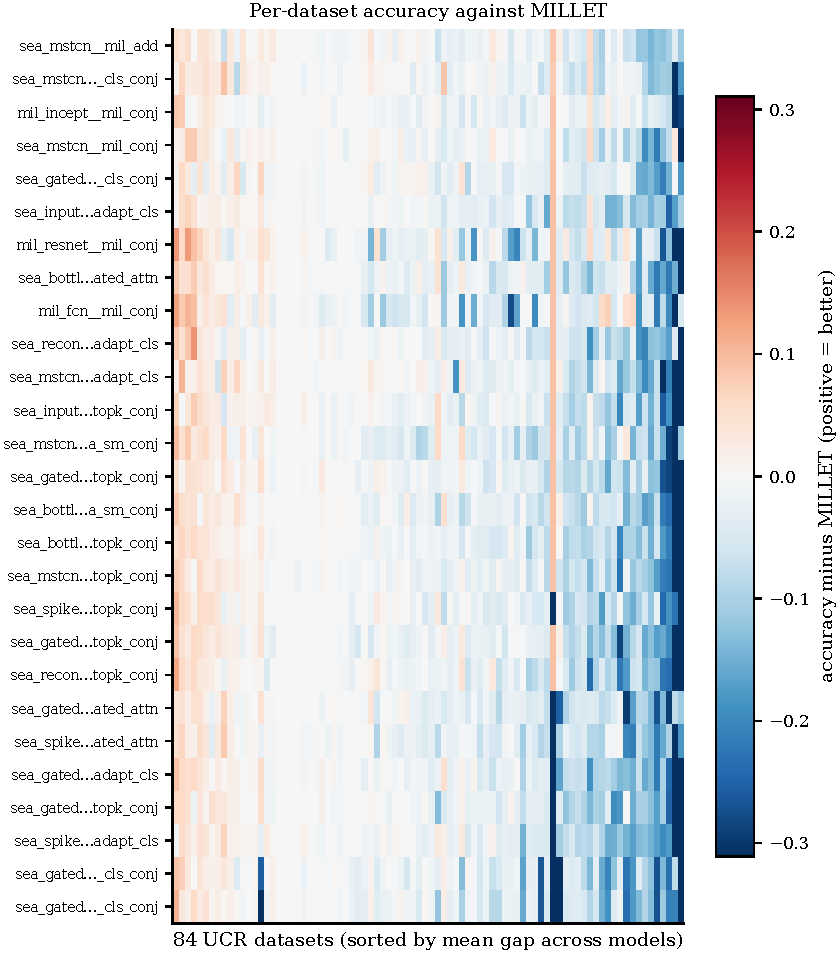
\includegraphics[width=\linewidth]{results/paper_figures/03_appendix/appendix_dataset_model_heatmap_accuracy}
  \caption{Per-dataset accuracy difference from the published MILLET results for every fully-swept model (27 models x 84 datasets). Blue is better than the baseline, red is worse, white is equal. Datasets are ordered by mean difference, so systematic strengths and weaknesses appear as vertical bands. Dataset names are omitted for space; the ordering is in the accompanying CSV.}
  \label{fig:appendix_dataset_model_heatmap_accuracy}
\end{figure*}

% Per-dataset accuracy distribution
% Question answered: How consistent is each model across datasets, not just on average?
\begin{figure}[t]
  \centering
  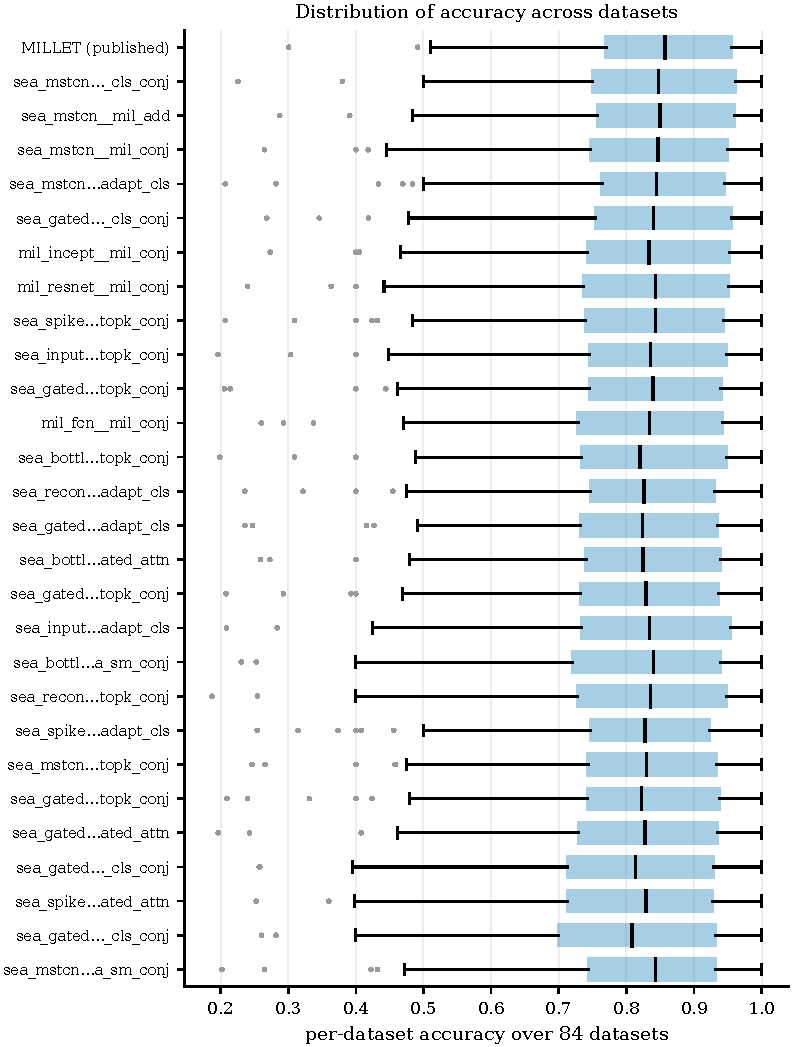
\includegraphics[width=\linewidth]{results/paper_figures/03_appendix/appendix_accuracy_distribution}
  \caption{Distribution of accuracy across 84 datasets for each fully-swept model, ordered by average rank. The box spans the interquartile range and the line is the median, so consistency is visible alongside central tendency. Note that this shows variation across DATASETS: each model was trained once, so these boxes do not represent run-to-run variance.}
  \label{fig:appendix_accuracy_distribution}
\end{figure}
